% 
% Annual Cognitive Science Conference
% Sample LaTeX Paper -- Proceedings Format
% 

% Original : Ashwin Ram (ashwin@cc.gatech.edu)       04/01/1994
% Modified : Johanna Moore (jmoore@cs.pitt.edu)      03/17/1995
% Modified : David Noelle (noelle@ucsd.edu)          03/15/1996
% Modified : Pat Langley (langley@cs.stanford.edu)   01/26/1997
% Latex2e corrections by Ramin Charles Nakisa        01/28/1997 
% Modified : Tina Eliassi-Rad (eliassi@cs.wisc.edu)  01/31/1998
% Modified : Trisha Yannuzzi (trisha@ircs.upenn.edu) 12/28/1999 (in process)
% Modified : Mary Ellen Foster (M.E.Foster@ed.ac.uk) 12/11/2000
% Modified : Ken Forbus                              01/23/2004
% Modified : Eli M. Silk (esilk@pitt.edu)            05/24/2005
% Modified : Niels Taatgen (taatgen@cmu.edu)         10/24/2006
% Modified : David Noelle (dnoelle@ucmerced.edu)     11/19/2014

%% Change "letterpaper" in the following line to "a4paper" if you must.

\documentclass[10pt,letterpaper]{article}

\usepackage{cogsci}
\usepackage{pslatex}
\usepackage{apacite}
\usepackage{graphicx}
%\graphicspath{plots/}
%\usepackage{float}
\usepackage[section]{placeins}

\title{Developmental Change in the Relationship Between Lexical and Grammatical Acquisition}
 
\author{{\large \bf Mika Braginsky} \\
  \texttt{mikabr@stanford.edu} \\
  Department of Psychology \\
  Stanford University
  \And {\large \bf Daniel Yurovsky} \\
  \texttt{yurovsky@stanford.edu} \\
  Department of Psychology \\
  Stanford Uiversity
    \And {\large \bf Virginia Marchman} \\
    \texttt{marchman@stanford.edu} \\
  Department of Psychology \\
  Stanford Uiversity
    \And {\large \bf Michael C. Frank}\\
    \texttt{mcfrank@stanford.edu} \\
  Department of Psychology \\
  Stanford Uiversity}


\begin{document}

\maketitle

\begin{abstract}
Lorem ipsum dolor sit amet, consectetur adipiscing elit. Aenean volutpat eu dui et bibendum. Curabitur ut neque vel nulla dignissim pellentesque. Sed lacinia mi sit amet libero pellentesque cursus. Sed ut vulputate augue. Quisque porta leo pulvinar, congue massa at, dapibus metus. Maecenas malesuada eleifend metus quis sagittis. Vivamus fermentum rhoncus sodales. Aliquam vitae pharetra lacus. Duis quis leo id orci porttitor elementum. Integer dictum ex enim, sed convallis tellus ultricies sed. Vestibulum pretium convallis fermentum. Sed ac sapien et magna dignissim aliquet et sed turpis.

\textbf{Keywords:} 
foo; bar; baz
\end{abstract}

\section{Introduction}

[Intro material written by Mike:]
Does abstract structure in language emerge from the interaction of individual words, or are syntactic structures represented separately? On lexicalist theories of grammatical development, syntactic structure emerges from graded generalizations on the basis of lexical items and there may be little or no representation of syntactic rules or regularities per se, at least early in development (Tomasello, 2000; 2003). Even if syntactic structures are eventually represented, these representations should be directly related to their support in more concrete lexical structure (Bannard et al., 2009; Bod, 2010??). In contrast, on theories like principles and parameters, grammar is predicted to emerge independently from lexical knowledge and on its own (largely maturational) timetable. On these theories, older children should have more syntactic competence, largely independent from the amount of language input they receive and hence from the size of their vocabulary.

Developmental data can help resolve this conflict by providing estimates of the relationship between grammar, lexicon, and age. Indeed, in a now-classic set of analyses, Bates \& Goodman (1995) showed a systematic relationship between ...

[Intro material written by Mika:]
[Sentence about how all grammar generalizations must involve both input and internal stuff]. However, theories of grammatical development differ in the role that they assign to experience and internal processes and the emphasis that they place on one or the other. One one hand, in the more nativist and domain-specific tradition [stuff about generative grammar and Principles and Parameters (cite Atoms of Language and Chomsky); basically everything is maturation]. On the other hand, [stuff about emergentism and lexicalist grammar (cite Bates and Goodman 1999 and maybe some Tomasello)].

[Stuff about how those theories make different predictions and how those predictions can be explored in empirical studies of lexicon-grammar relationship. If there's age-related change, functions should be different at different age points. If there's no age-related change, functions should be the same.]

[What functions? How two relate lexicon to grammatical development? Two different metrics: 1) usage of grammatical forms and constructions; 2) composition of lexicon by grammatical function.]

[How to measure any of these things? CDI of course! Justification for CDI (Fenson, 1994), justification for complexity section (Dale, 1991; Dale et al, 1989) and word form section (???).]

[Previous work on lexicon-grammar: well-established tight connection between lexicon and grammar, same non-linear function everywhere in English (Bates et al, 1994; Fenson et al, 1994, Italian (Caselli, Casadio, Bates, 2000), Hebrew (Maital, Dromi, Sagi, Bornstein, 2000), Icelandic (Thordardottir, Weismer, Evans, 2002), Spanish (Jackson-Maldonado et al, 2003)]. [Bates and Goodman (1999) conclude that grammar is entirely predictable from lexicon. But we find additional effect of age, suggesting there's a tight link but there's also something developmental going on.]

[Previous work on lexical composition: English (Bates et al, 1994), other languages (???).]

\clearpage

\section{General Methods}

\subsection{CDI Form Database}:

[Talk about wordbank, all the sources of our data, give some numbers of kids.]

[Talk in more detail about the CDI and the specifics of the languages and forms.]

\subsection{Data Sources}


\subsection{CDI Measures}

In general CDI forms contain both vocabulary checklists and other questions relevant to the child's ...

\section{Developmental Interactions in Syntax and Morphology}



\begin{figure*}[t]
\begin{center}
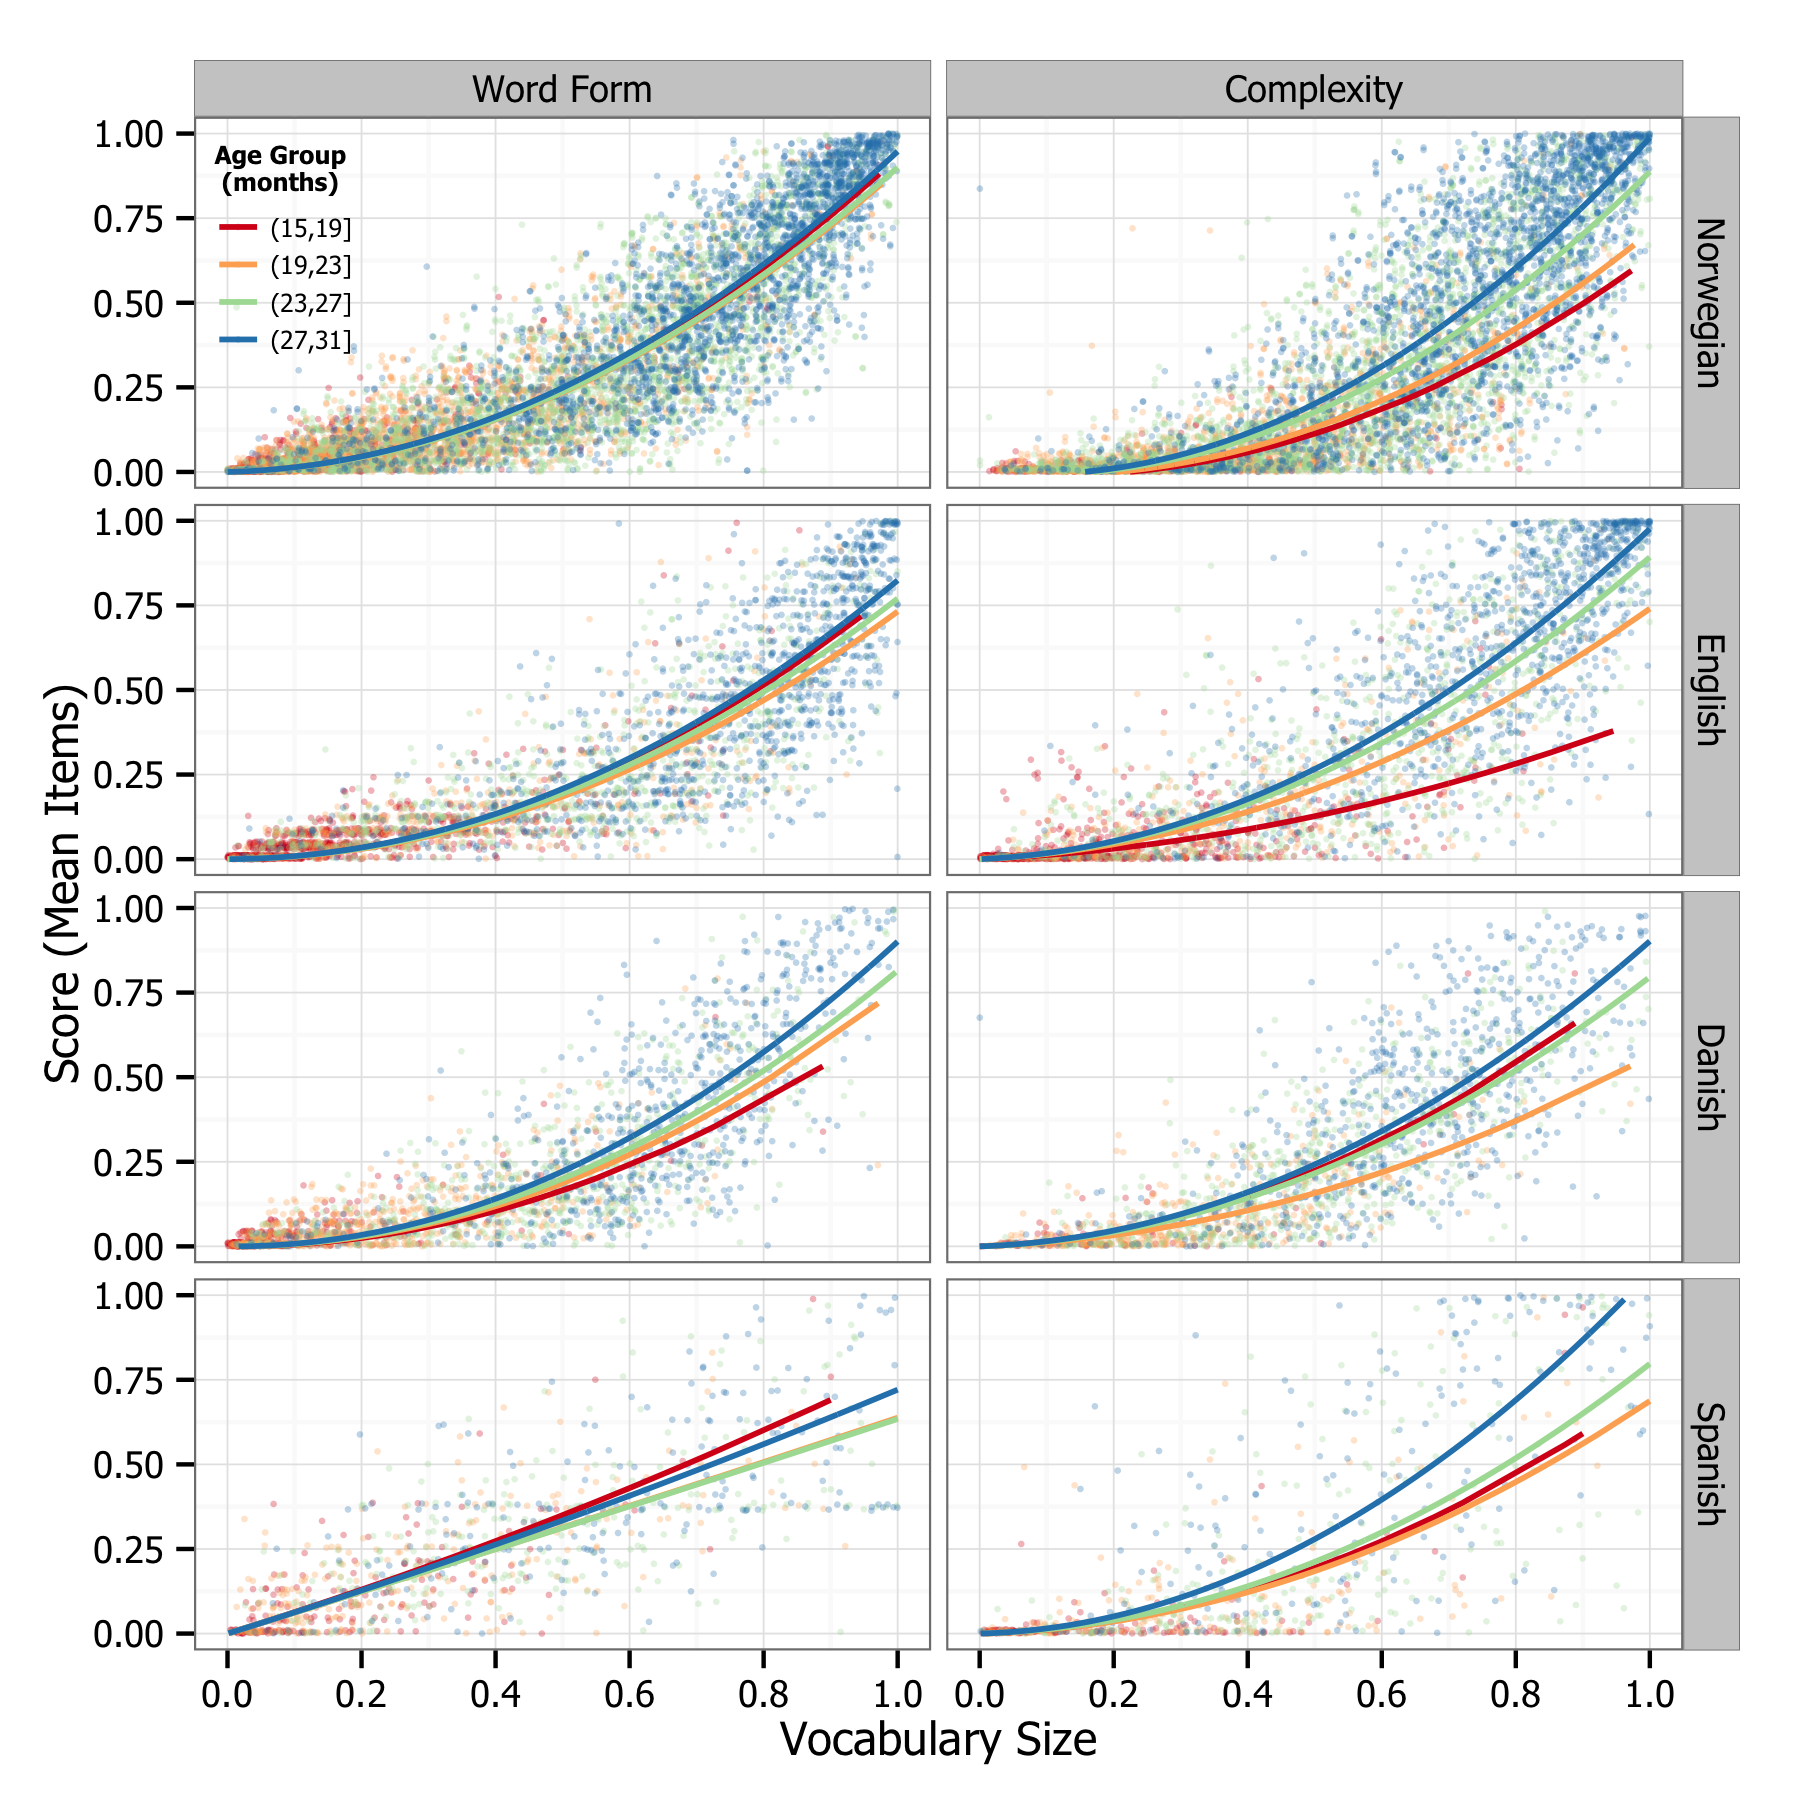
\includegraphics[scale=0.8]{plots/grammar.png}
\end{center}
\caption{Grammar!} 
\label{grammar}
\end{figure*}

\begin{figure}[t]
\begin{center}
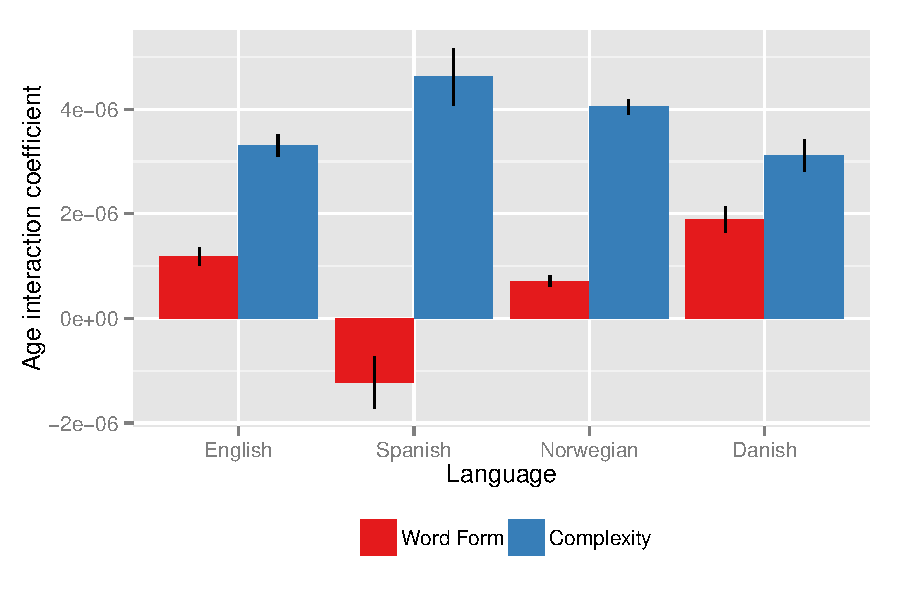
\includegraphics[width=\linewidth]{plots/coeffs}
\end{center}
\caption{Coefficients} 
\label{coeffs}
\end{figure}

% \begin{figure}[h]
% \begin{center}
% 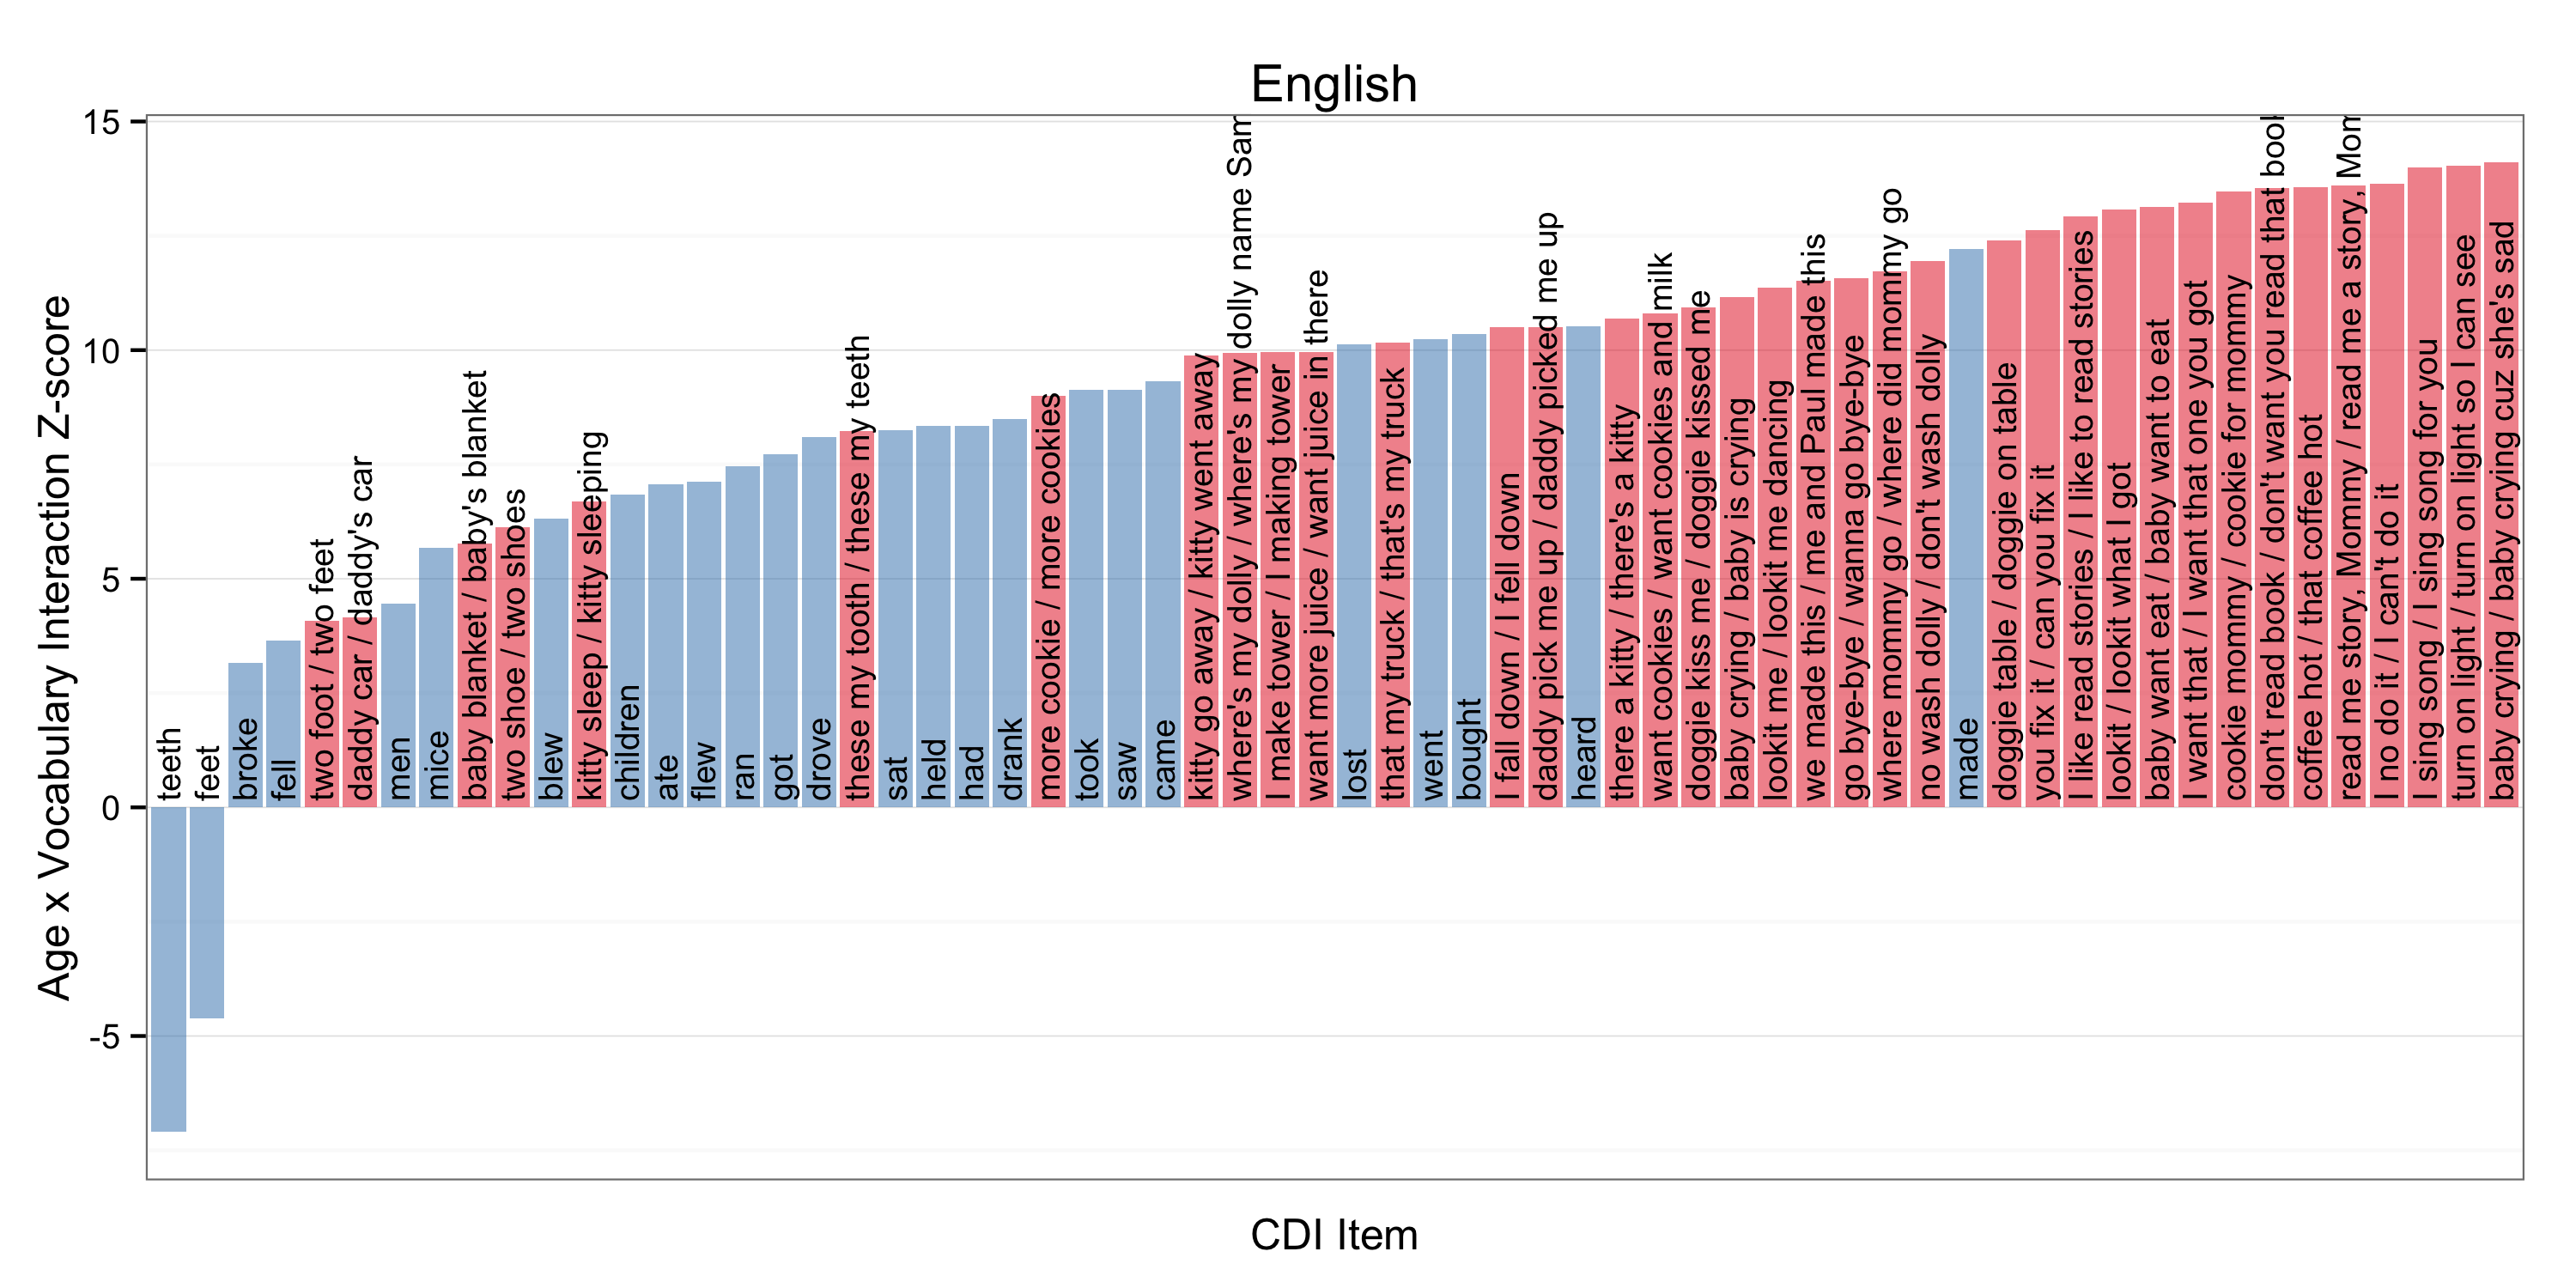
\includegraphics[width=\linewidth]{plots/english_interactions}
% \end{center}
% \caption{English} 
% \label{english_interactions}
% \end{figure}

% \begin{figure}[h]
% \begin{center}
% 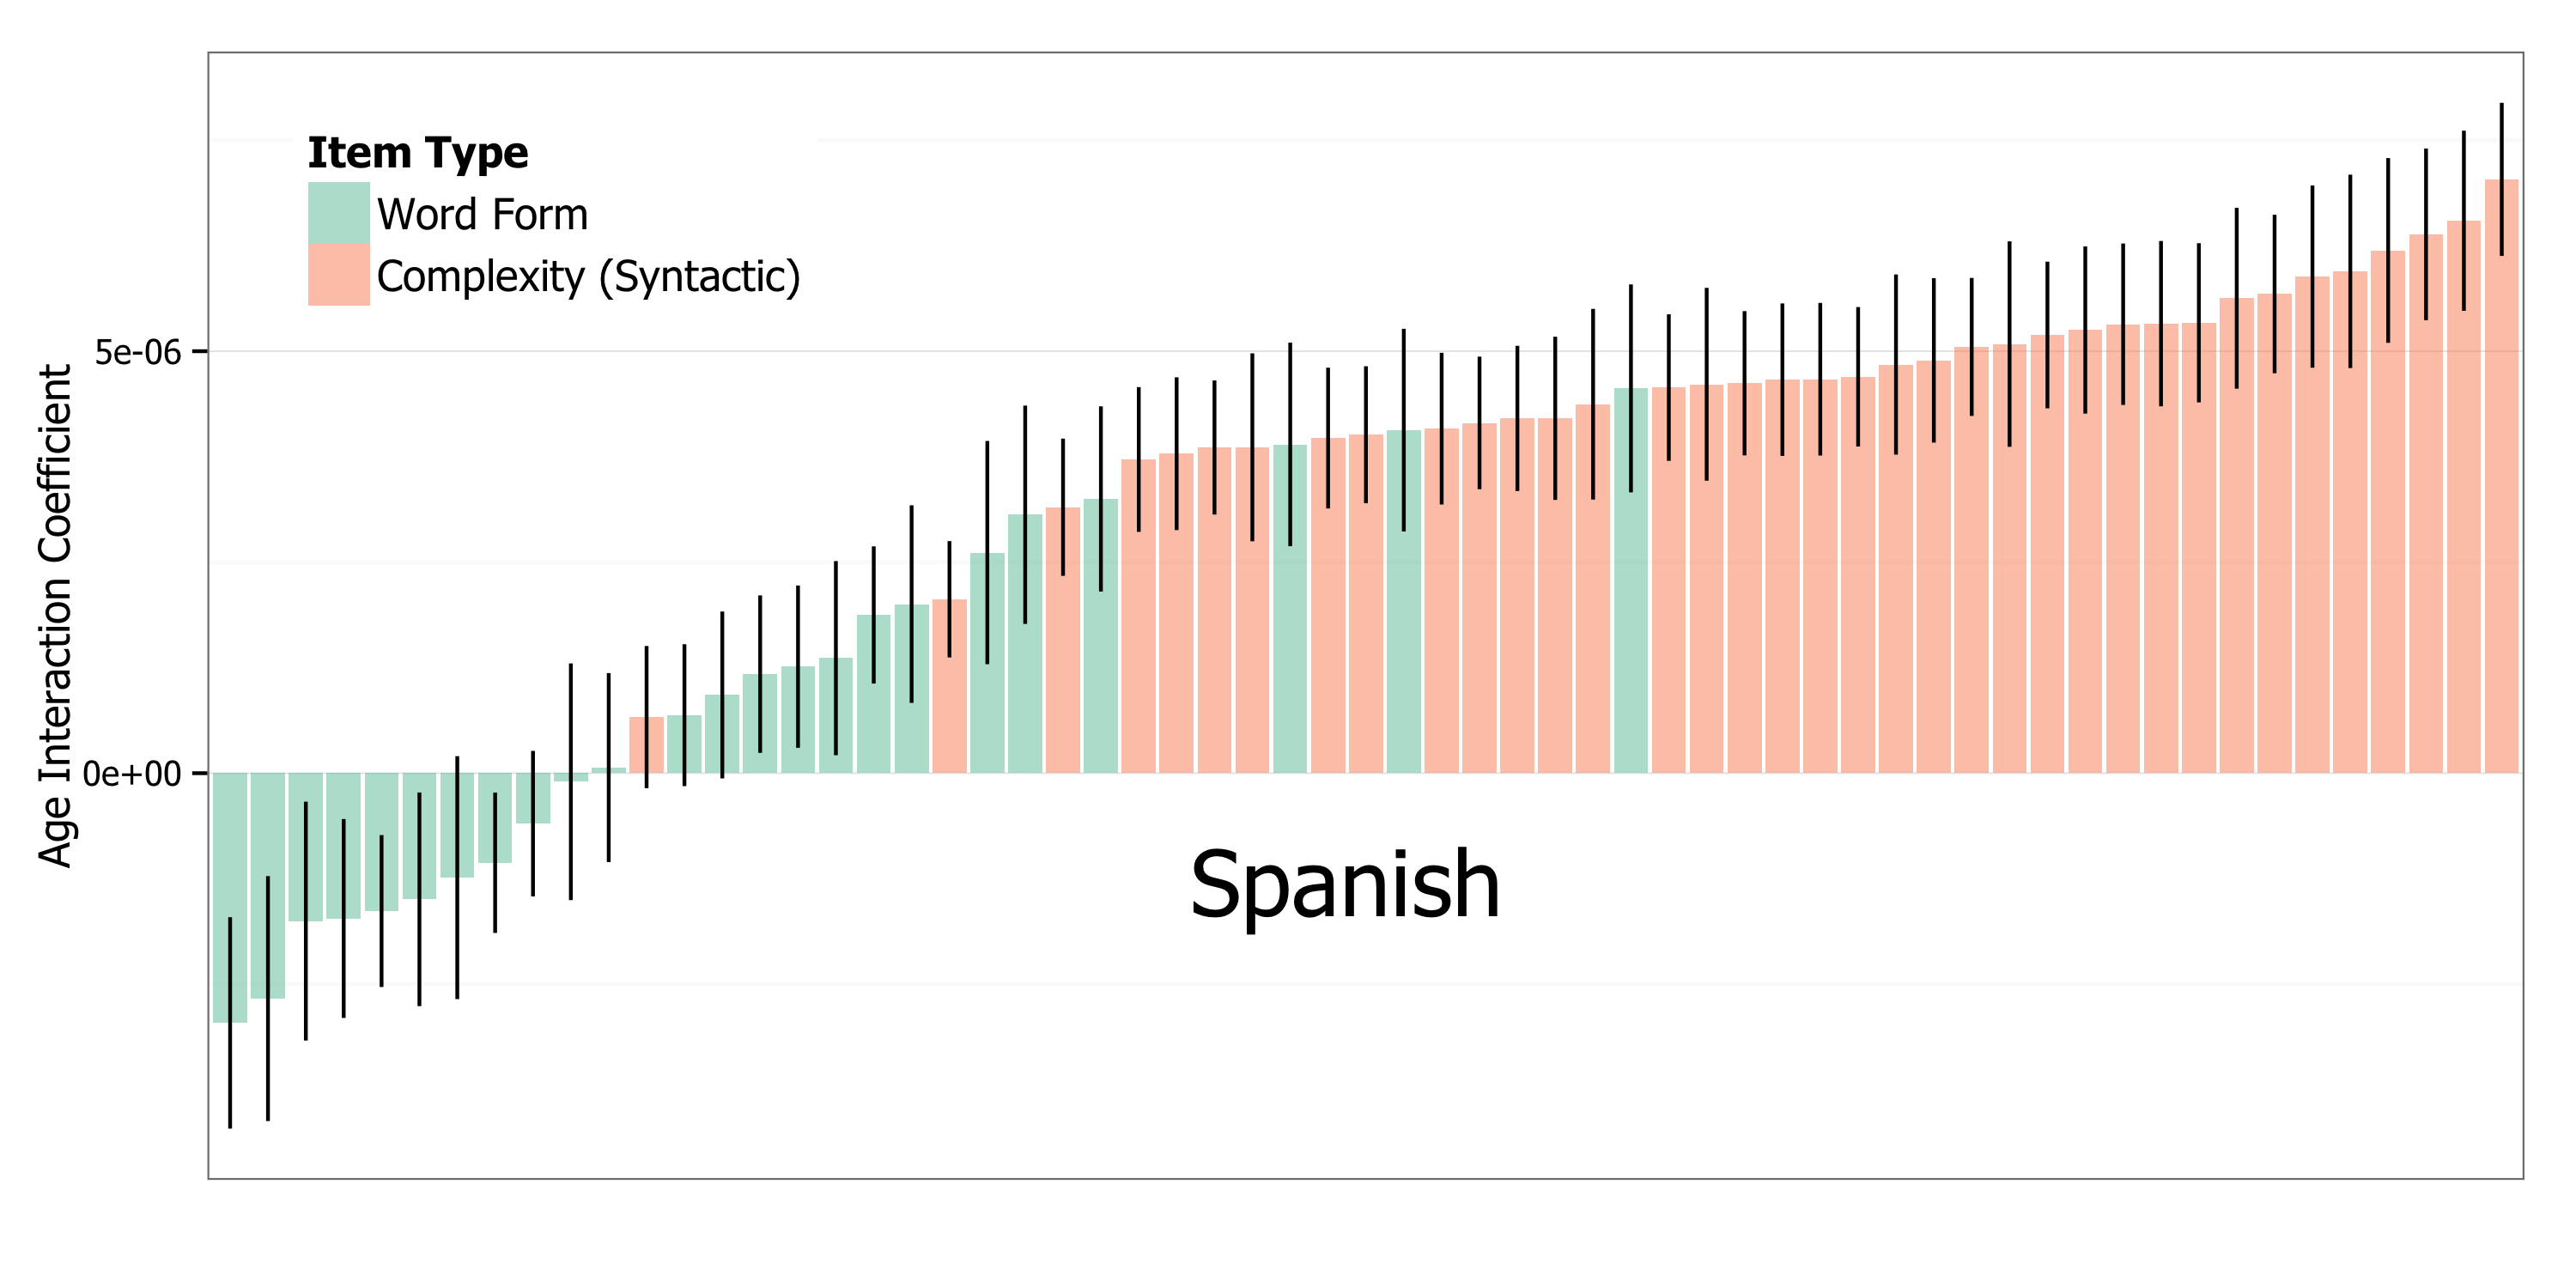
\includegraphics[width=\linewidth]{plots/spanish_interactions}
% \end{center}
% \caption{Spanish} 
% \label{spanish_interactions}
% \end{figure}

% \begin{figure}[h]
% \begin{center}
% 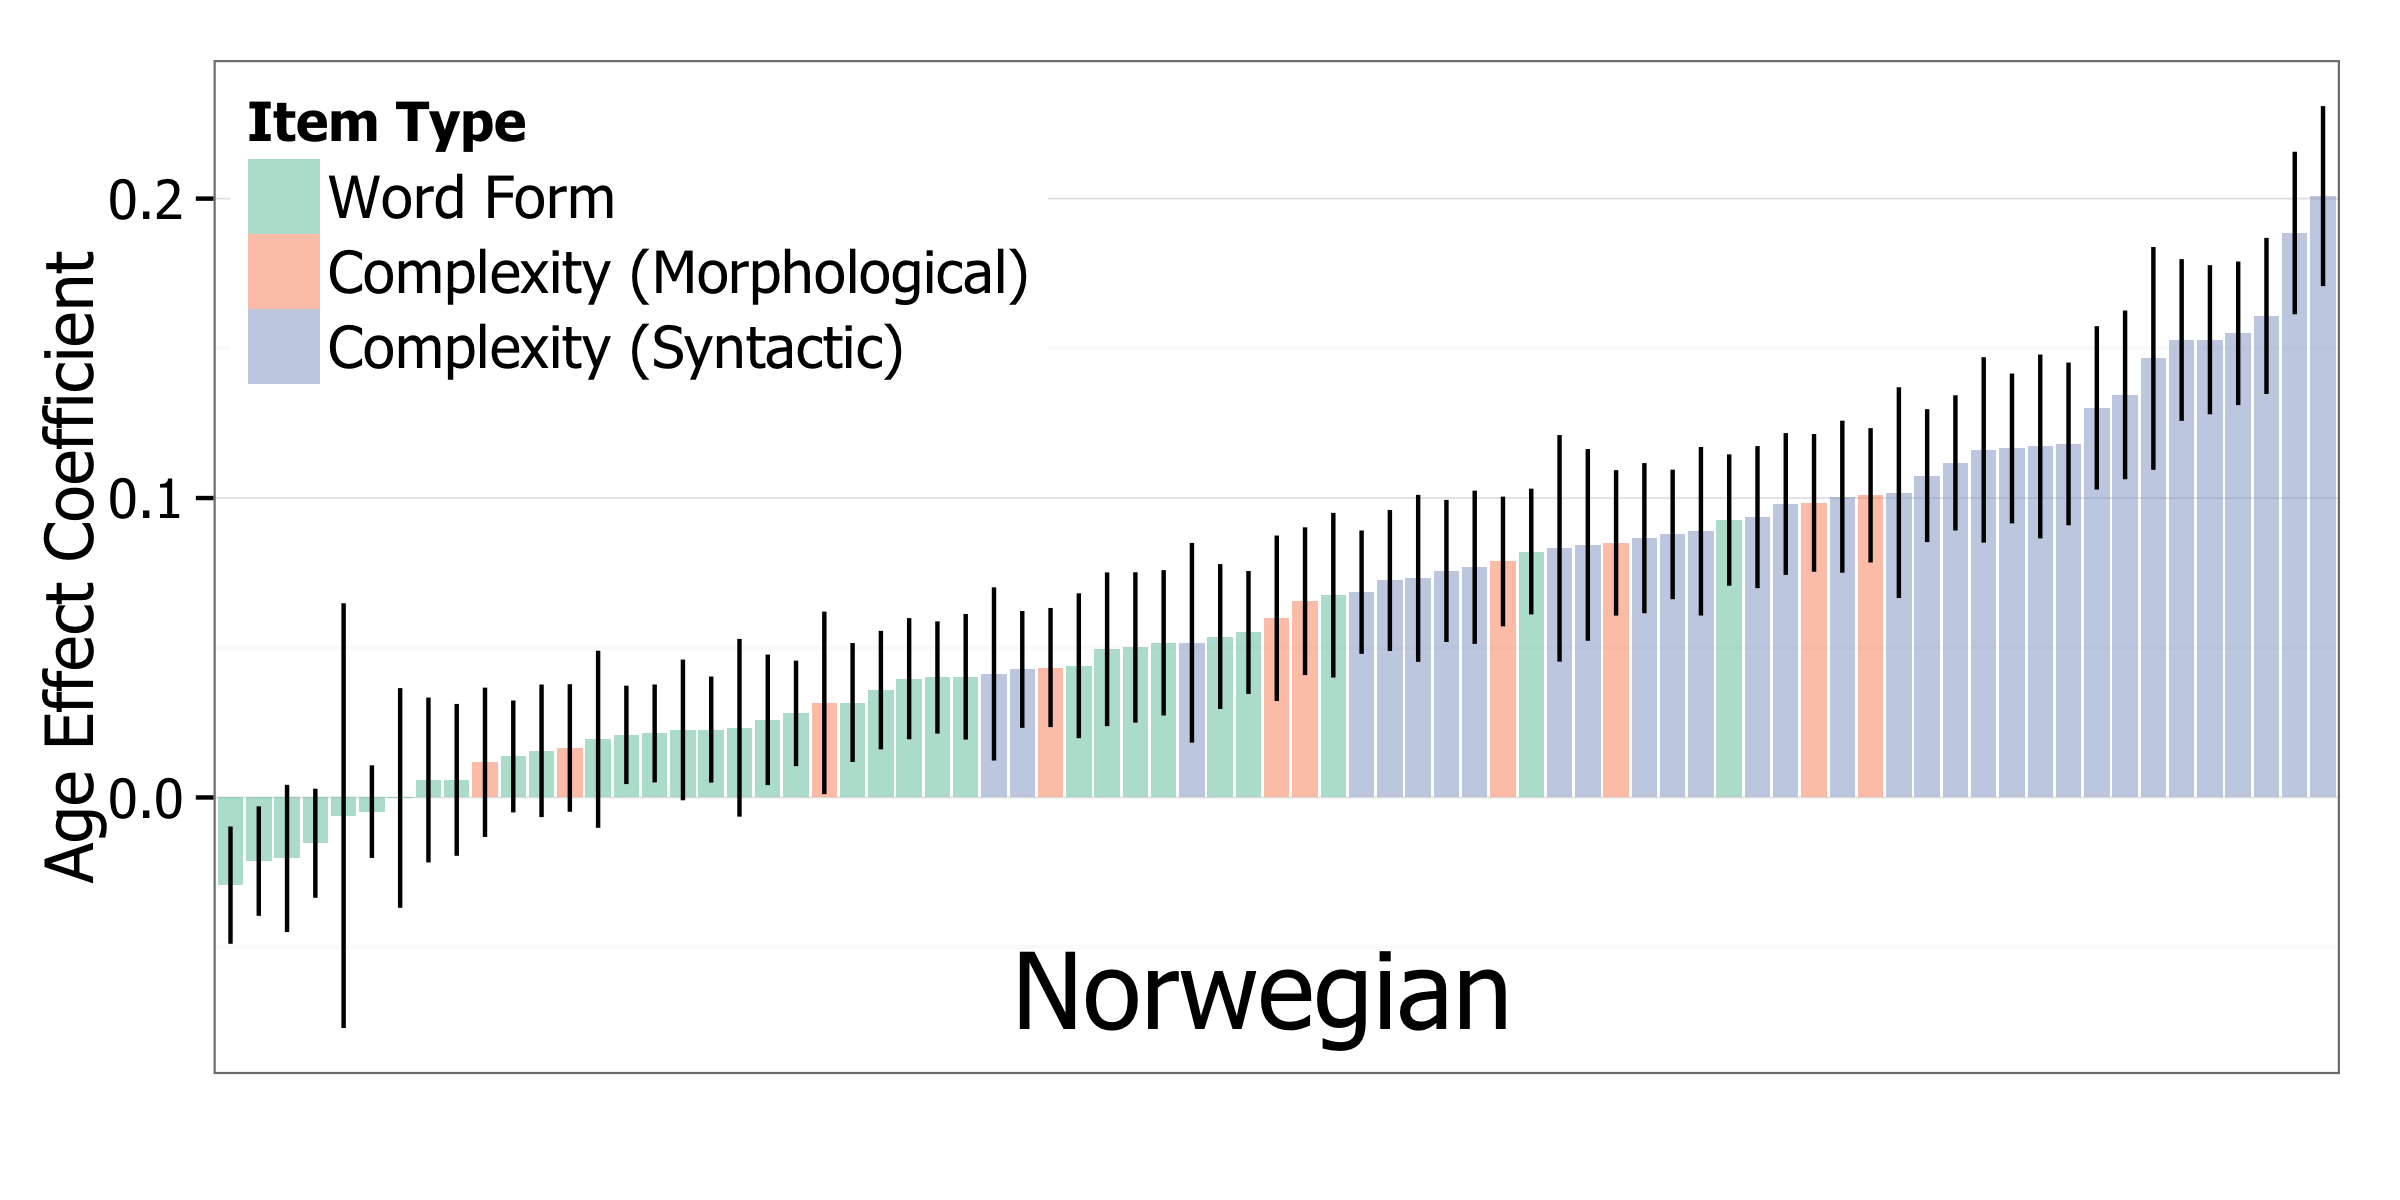
\includegraphics[width=\linewidth]{plots/norwegian_interactions}
% \end{center}
% \caption{Norwegian} 
% \label{norwegian_interactions}
% \end{figure}

% \begin{figure}[h]
% \begin{center}
% 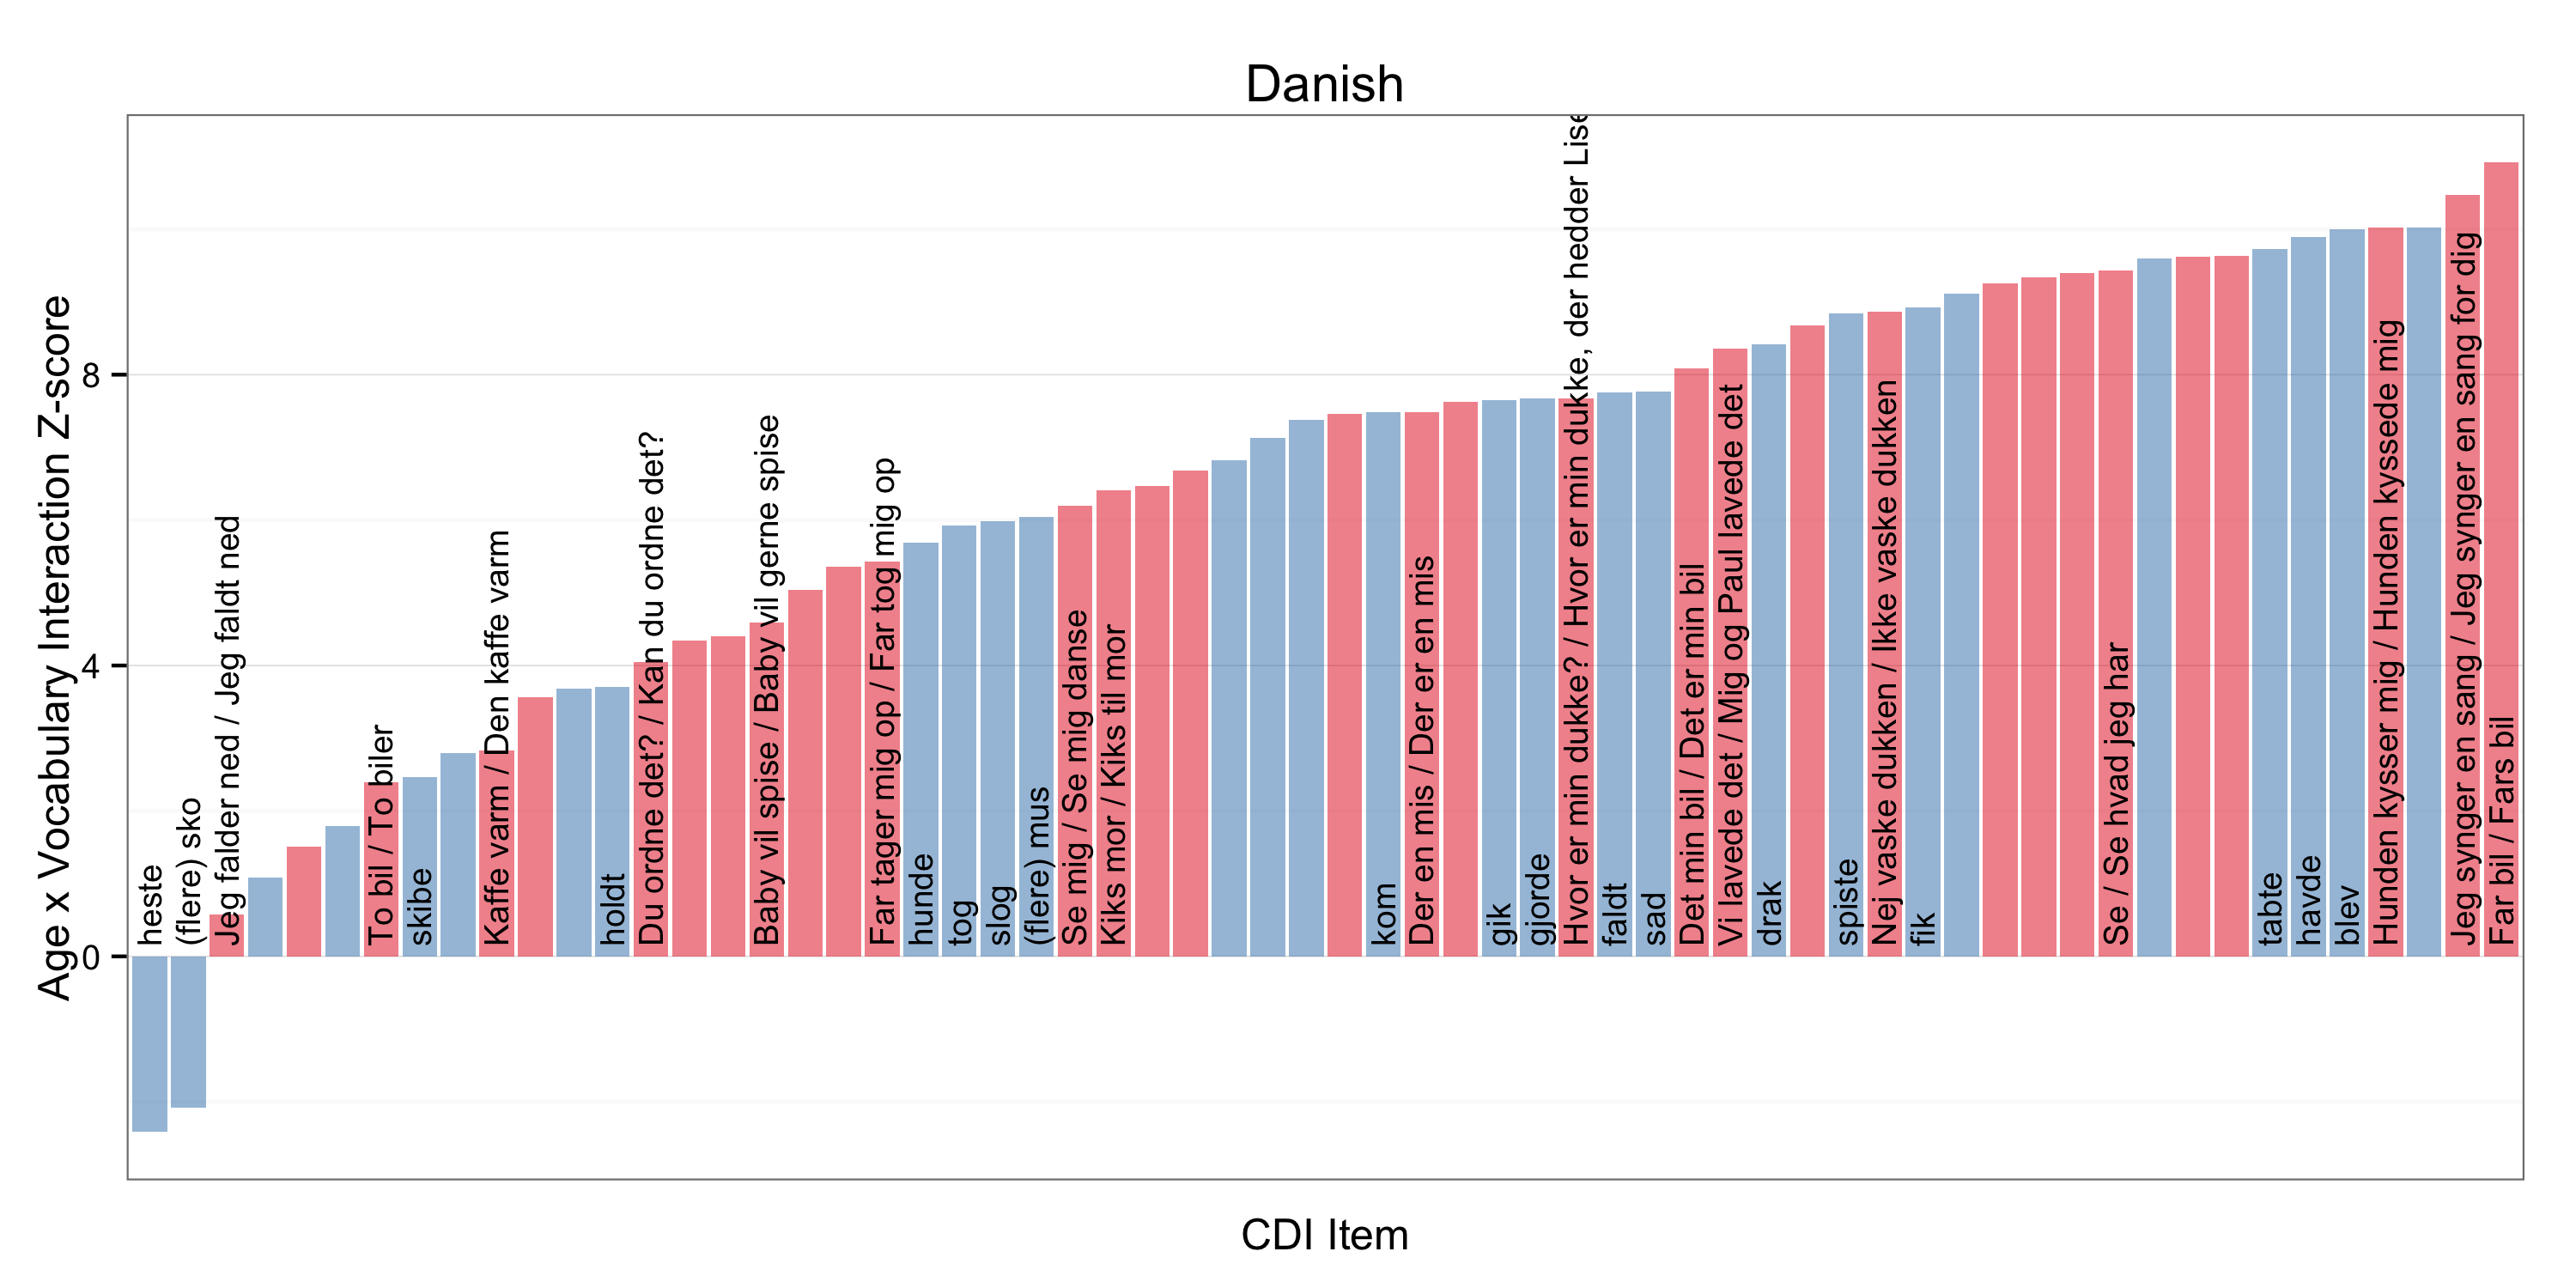
\includegraphics[width=\linewidth]{plots/danish_interactions}
% \end{center}
% \caption{Danish} 
% \label{danish_interactions}
% \end{figure}


[Introduce and scaffold results.]

\section{Developmental Interactions in Vocabulary Composition}

Early vocabulary development is typically characterized by learning of names for caregivers and common objects, while l ater in development, children tend to increase their vocabulary by increasing the proportion of predicates (verbs and adjectives). This over-representation of nouns has been found across a number of analyses and in a variety of languages, though not all \cite{caselli1995}.\footnote{Differences in early vocabulary composition have been argued to emerge from typological differences (e.g., word order, subject drop), and from cultural practices (e.g., focus on picture book reading) \cite{tardif1999, gopnik1996, choi1995}---we are agnostic as to the source of this variability.} For our purposes we are interested in using these analyses of vocabulary composition to test for the same kind of age-related differences that we found in the complexity and word-form analyses reported above. 

We predict that the proportion of verbs in children's vocabulary should be relatively more affected by age than nouns. Concrete nouns are hypothesized to be learned initially from both co-occurrences between words \cite{yu2007b} and by social cues to reference to particular objects \cite{bloom2002}. On neither of these accounts should syntactic information be a primary information source (though of course syntax might be more informative for abstract nouns). In contrast, for verbs, syntax has been argued to be primary in meaningl learning. On the syntactic bootstrapping hypothesis \cite{gleitman1990,fisher1993}, verbs are learned by  mapping the syntactic structure of utterances to the thematic structure of observed events, for example by noticing that the subject of a sentence matches the agent in one particular ongoing event but not another (``the cat is fleeing the dog'' matches  {\sc flees(cat, dog)} but not {\sc chases(dog,cat)}). Thus, if syntactic development is related in some way to age, we should see larger age effects on verb representation than noun representation. 

\subsection{Analysis}


\begin{figure*}[t!]
\begin{center}
\includegraphics[scale=1]{plots/composition.png}
\end{center}
\caption{\label{fig:beans} Proportion of a particular CDI category, plotted by total vocabulary size. Each point shows an individual child, with color showing their noun, predicate, and function word vocabulary. Panels show different languages, and curves are smoothing functions using loess.} 

\end{figure*}


Each CDI form contains a mixture of words in different classes. We adopt the categorization of \citeA{bates1994}, who split words in nouns, predicates (adjectives, adverbs, and verbs), function words, and other words. Then for each child's vocabulary, we compute the proportion of the total words in each of these categories that they are reported to produce. This analysis yields a set of proportions for each child.

Again following \citeA{bates1994}, for each of the four languages in our sample, we plot these proportions against total vocabulary. These functions are shown in Figure \ref{fig:beans}: each dot represents an individual child's knowledge of a particular class, while curves show the relationship between that class and the entirety of the vocabulary. If categories grow independently of one another, these curves should approximate the diagonal. This pattern is not what either we or Bates and colleagues observe however: Across the languages in our sample, nouns are systematically over-represented in smaller vocabularies (shown by a curve that is above the diagonal), while function words---and to some extent, predicates---are under-represented. 

Next, we measure the contribution of age to vocabulary composition. We fit a linear model to all children's data for each word class, predicting word-class proportion as a linear and quadratic (FIXME) function of total vocabulary. We then investigated the interaction between total vocabulary and age. Because of our theoretical interest in the relationship between age and syntactic development, we focus here specifically on nouns and verbs. Figure \ref{fig:vocab_coefs} shows coefficients for each of these models across languages. In each model, the age-related interaction coefficient was substantially larger for verbs than for nouns. This asymmetry can be interpreted as evidence that for two vocabulary-matched children, the older would tend to have relatively more verbs than the younger, and this effect was larger for children with overall larger vocabularies.  

\subsection{Discussion}

We replicated previous analyses showing an over-representation of nouns in the developing lexicon and a relative under-representation of verbs. We additionally predicted that---if syntactic generalization was in some way tied to age---verbs would show relatively more influence than nouns. This prediction was confirmed across all four languages we examined. Thus, this analysis provides additional circumstantial evidence for the relationship between syntactic development and age, independent of the growth of the lexicon. 

\section{General Discussion}

\section{Acknowledgments}

Thanks to the MacArthur CDI Advisory Board, Doroth\'e Bleses, Kristian Kristofferson, Rune N\o rdgard, and the members of the Language and Cognition Lab. 

\section{References}

\bibliographystyle{apacite}

\setlength{\bibleftmargin}{.125in}
\setlength{\bibindent}{-\bibleftmargin}

\bibliography{CogSci}


\end{document}
